\documentclass{amsart}
\usepackage{amsmath}
\usepackage{amssymb}
\usepackage{amsthm}
%\usepackage{MnSymbol}
\usepackage{bm}
\usepackage{accents}
\usepackage{mathtools}
\usepackage{tikz}
\usetikzlibrary{calc}
\usetikzlibrary{decorations.pathmorphing,shapes}
\usetikzlibrary{automata,positioning}
\usepackage{tikz-cd}
\usepackage{forest}
\usepackage{braket} 
\usepackage{listings}
\usepackage{mdframed}
\usepackage{verbatim}
\usepackage{physics}
\usepackage{stmaryrd}
\usepackage{mathrsfs} 
\usepackage{stackengine} 
%\usepackage{/home/patrickl/homework/macaulay2}

%font
\usepackage[sc]{mathpazo}
\usepackage{eulervm}
\usepackage[scaled=0.86]{berasans}
\usepackage{inconsolata}
\usepackage{microtype}

%CS packages
\usepackage{algorithmicx}
\usepackage{algpseudocode}
\usepackage{algorithm}

% typeset and bib
\usepackage[english]{babel} 
\usepackage[utf8]{inputenc} 
\usepackage[T1]{fontenc}
%\usepackage[backend=biber, style=alphabetic]{biblatex}
\usepackage[bookmarks, colorlinks, breaklinks]{hyperref} 
\hypersetup{linkcolor=black,citecolor=black,filecolor=black,urlcolor=black}
\usepackage{graphicx}
\graphicspath{{./}}

% other formatting packages
\usepackage{float}
\usepackage{booktabs}
\usepackage[shortlabels]{enumitem}
\usepackage{csquotes}
%\usepackage{titlesec}
%\usepackage{titling}
%\usepackage{fancyhdr}
%\usepackage{lastpage}
\usepackage{parskip}

\usepackage{lipsum}

% delimiters
\DeclarePairedDelimiter{\gen}{\langle}{\rangle}
\DeclarePairedDelimiter{\floor}{\lfloor}{\rfloor}
\DeclarePairedDelimiter{\ceil}{\lceil}{\rceil}


\newtheorem{thm}{Theorem}[section]
\newtheorem{cor}[thm]{Corollary}
\newtheorem{prop}[thm]{Proposition}
\newtheorem{lem}[thm]{Lemma}
\newtheorem{conj}[thm]{Conjecture}
\newtheorem{quest}[thm]{Question}

\theoremstyle{definition}
\newtheorem{defn}[thm]{Definition}
\newtheorem{defns}[thm]{Definitions}
\newtheorem{con}[thm]{Construction}
\newtheorem{exm}[thm]{Example}
\newtheorem{exms}[thm]{Examples}
\newtheorem{notn}[thm]{Notation}
\newtheorem{notns}[thm]{Notations}
\newtheorem{addm}[thm]{Addendum}
\newtheorem{exer}[thm]{Exercise}

\theoremstyle{remark}
\newtheorem{rmk}[thm]{Remark}
\newtheorem{rmks}[thm]{Remarks}
\newtheorem{warn}[thm]{Warning}
\newtheorem{sch}[thm]{Scholium}


% unnumbered theorems
\theoremstyle{plain}
\newtheorem*{thm*}{Theorem}
\newtheorem*{prop*}{Proposition}
\newtheorem*{lem*}{Lemma}
\newtheorem*{cor*}{Corollary}
\newtheorem*{conj*}{Conjecture}

% unnumbered definitions
\theoremstyle{definition}
\newtheorem*{defn*}{Definition}
\newtheorem*{exer*}{Exercise}
\newtheorem*{defns*}{Definitions}
\newtheorem*{con*}{Construction}
\newtheorem*{exm*}{Example}
\newtheorem*{exms*}{Examples}
\newtheorem*{notn*}{Notation}
\newtheorem*{notns*}{Notations}
\newtheorem*{addm*}{Addendum}


\theoremstyle{remark}
\newtheorem*{rmk*}{Remark}

% shortcuts
\newcommand{\Ima}{\mathrm{Im}}
\newcommand{\A}{\mathbb{A}}
\newcommand{\G}{\mathbb{G}}
\newcommand{\N}{\mathbb{N}}
\newcommand{\R}{\mathbb{R}}
\newcommand{\C}{\mathbb{C}}
\newcommand{\Z}{\mathbb{Z}}
\newcommand{\Q}{\mathbb{Q}}
\renewcommand{\k}{\Bbbk}
\renewcommand{\P}{\mathbb{P}}
\newcommand{\M}{\overline{M}}
\newcommand{\g}{\mathfrak{g}}
\newcommand{\h}{\mathfrak{h}}
\newcommand{\n}{\mathfrak{n}}
\renewcommand{\b}{\mathfrak{b}}
\newcommand{\ep}{\varepsilon}
\newcommand*{\dt}[1]{%
   \accentset{\mbox{\Huge\bfseries .}}{#1}}
%\renewcommand{\abstractname}{Official Description}
\newcommand{\mc}[1]{\mathcal{#1}}
% \newcommand{\msc}[1]{\mathscr{#1}}
\newcommand{\T}{\mathbb{T}}
\newcommand{\mf}[1]{\mathfrak{#1}}
\newcommand{\mr}[1]{\mathrm{#1}}
\newcommand{\ms}[1]{\mathsf{#1}}
\newcommand{\ol}[1]{\overline{#1}}
\newcommand{\ul}[1]{\underline{#1}}
\newcommand{\wt}[1]{\widetilde{#1}}
\newcommand{\wh}[1]{\widehat{#1}}
\renewcommand{\div}{\operatorname{div}}
\newcommand{\1}{\mathbf{1}}
\newcommand{\2}{\mathbf{2}}
\newcommand{\3}{\mathbf{3}}
\newcommand{\I}{\mathrm{I}}
\newcommand{\II}{\mr{I}\hspace{-1.3pt}\mr{I}}
\newcommand{\III}{\mr{I}\hspace{-1.3pt}\mr{I}\hspace{-1.3pt}\mr{I}}

\DeclareMathOperator{\Der}{Der}
\DeclareMathOperator{\Tor}{Tor}
\DeclareMathOperator{\Hom}{Hom}
\DeclareMathOperator{\End}{End}
\DeclareMathOperator{\Ext}{Ext}
\DeclareMathOperator{\ad}{ad}
\DeclareMathOperator{\Aut}{Aut}
\DeclareMathOperator{\Rad}{Rad}
\DeclareMathOperator{\Pic}{Pic}
\DeclareMathOperator{\supp}{supp}
\DeclareMathOperator{\Supp}{Supp}
\DeclareMathOperator{\depth}{depth}
\DeclareMathOperator{\sgn}{sgn}
\DeclareMathOperator{\spec}{Spec}
\DeclareMathOperator{\Spec}{Spec}
\DeclareMathOperator{\proj}{Proj}
\DeclareMathOperator{\Proj}{Proj}
\DeclareMathOperator{\ord}{ord}
\DeclareMathOperator{\Div}{Div}
\DeclareMathOperator{\Bl}{Bl}

\title{The HOMFLY polynomial and enumerative geometry}
\author{Patrick Lei}
\date{October 5, 2021}

\begin{document}
    
\maketitle

\begin{abstract}
    We will begin by introducing Pandharipande-Thomas theory and computing the equivariant vertex. After that, we will sketch a proof of the Oblomkov-Shende conjecture following Maulik. In particular, we will give a proof of invariance of certain PT invariants under flops.
\end{abstract}

\section{Introduction}%
\label{sec:introduction}

Let $C \subset \C^2$ be a reduced curve and suppose $p \in C$ is an (isolated) singularity. Then define a constructible function $m \colon C_p^{[n]} \to \N$ given by $m([Z])$ being the number of generators of the ideal $I_{Z,p} \subset \mc{O}_{C,p}$. Now consider the generating function
\[ \ms{Z}_{C,p}(v, w) = \sum_{n \geq 0} s^{2n} \int_{C_p^{[n]}} (1-v^2) \dd{\chi} = \sum_{n \geq 0} s^{2n} \sum_k k \chi_{\mr{top}}(f^{-1}(k)). \]

Additionally, taking a small $S^3$ around $p \in \C^2$ and intersecting with $C$ gives us a link $\mc{L}_{C,p}$. Recall the HOMFLY polynomial $\ms{P}(\mc{L}; v, s) \in \Z[v^{\pm}, {(s-s^{-1})}^{\pm}]$. If $\mu$ is the Milnor number of the singularity (for example, the middle Betti number of the Milnor fiber), then the Oblomkov-Shende conjecture is
\begin{thm}[Maulik]
    \[ \ms{P}(\mc{L}_{C,p}; v,s) = {\qty(\frac{v}{w})}^{\mu - 1} \ms{Z}_{C,p}(v,s). \]
\end{thm}

The proof of this result relates both sides of the equality to enumerative geometry, and in particular Pandharipande-Thomas, or stable pairs, curve counting. In this lecture, we will (attempt to) sketch a proof of the Oblomkov-Shende conjecture, but first we will introduce PT theory to familiarize ourselves with the objects involved in the proof.

\begin{rmk}
    Maulik proves everything for a colored version of the HOMFLY polynomial, but here we will only work with uncolored data, which corresponds to all partitions being $(1)$.
\end{rmk}

\section{Introduction to PT Theory}%
\label{sec:introduction_to_pt_theory}

In this part, we are following the papers \textit{Curve counting via stable pairs in the derived category} and \textit{Stable pairs and BPS invariants} by Pandharipande and Thomas.

Let $X$ be a smooth threefold and $\beta \in H_2(X, \Z)$. The \textit{PT moduli space} $P_n(X, \beta)$ parameterizes two-term complexes
\[ \mc{O}_X \xrightarrow{s} \mc{F}, \]
where $\mc{F}$ is a pure $1$-dimensional sheaf supported on a Cohen-Macaulay subcurve of $X$, $s$ has $0$-dimensional cokernel, $\chi(\mc{F}) = n$, and $[\supp F] = \beta$. The space $P_n(X, \beta)$ has a virtual fundamental class coming from the deformation theory of complexes in the derived category. Here, note that the deformation theory of $(\mc{F}, s)$ (really of the corresponding complex $\mc{I}^{\bullet}$) is given by
\[ \Ext^0(\mc{I}^{\bullet}, \mc{F}) \to \Ext^1(\mc{I}^{\bullet}, \mc{F}) = {\Ext^1(\mc{I}^{\bullet}, \mc{I}^{\bullet})}_0 \to {\Ext^2(\mc{I}^{\bullet}, \mc{I}^{\bullet})}_0 \]
and the virtual fundamental class lives in dimension
\[ c_{\beta} \coloneqq \int_{\beta} c_1(X). \]
In particular, for a Calabi-Yau threefold, $c_{\beta} = 0$. Given this data, we may define the \textit{PT invariant}
\[ P_{n, \beta} \coloneqq \int_{{[P_n(X, \beta)]}^{\mr{vir}}} 1. \]
and the $PT$ partition function
\[ \ms{Z}_{PT, \beta}(q) = \sum P_{n, \beta} q^n. \]

There is an alternative way to compute the PT invariants for $X$ a projective Calabi-Yau threefold, due to Behrend (originally done for DT theory). In this case, the moduli space is actually a projective scheme, and if $P_n(X, \beta)$ is smooth everywhere, then
\[ P_{n, \beta} = {(-1)}^{\dim P_n(X, \beta)} \chi_{\mr{top}}(P_n(X, \beta)). \]
Of course, moduli spaces are almost never smooth for nontrivial moduli problems, so instead, we have
\begin{prop}[Behrend]
    There exists an integer-valued constructible function $\chi_B$ such that
    \[ P_{n, \beta} = \int_{P_n(X, \beta)} \chi_B \coloneqq \sum_{n \in \Z} n \chi_{\mr{top}}({(\chi_B)}^{-1}(n)). \]
\end{prop}

\section{A computation in PT theory}%
\label{sec:a_computation_in_pt_theory}

This computation comes from \textit{The $3$-fold vertex via stable pairs} by Pandharipande and Thomas.

We will now compute the $T$-equivariant PT vertex of $\C^3$ (this is the local model for toric varieties) to give us all a feel for this enumerative theory. First, we need to define some combinatorial data. Let $\mu = (\mu_1, \mu_2, \mu_3)$ be a triple of partitions. Then there exists a unique minimal $T$-fixed subscheme $C_{\mu}$ with outgoing partitions the $\mu_i$ (simply take the curves $C_{\mu_i}$ given by the three partitions and take the union), whose ideal we will denote $\mc{I}_{\mu}$. Then we define
\[ M = \bigoplus_{i=1}^3 {(\mc{O}_{C_{\mu_i}})}_{x_i} \eqqcolon \bigoplus_{i=1}^3 M_i. \]
Every $T$-invariant pair $(\mc{F}, s)$ on $\C^3$ corresponds to a finitely-generated $T$-invariant submodule
\[ Q \subset M/\ev{(1,1,1)}, \]
and we will now give a combinatorial description of such submodules.

For each $\mu^i$, we may consider the module $M_i$ as an infinite cylinder $\mr{Cyl}_i \subset \Z^3$ (extending in both directions). Then for every $w \in \Z^3$, consider the vectors $\1_w, \2_w, \3_w$ representing $w$ in each copy of $\Z^3$ (for each of the $M_i$). Clearly $x_1$ shifts $w$ by $(1,0,0)$ and similarly for $x_2, x_3$. We will now consider the decomposition of the union of the $\mr{Cyl}_i$ into the following types:
\begin{itemize}
    \item Type $\I^+$ are those which have only nonnegative coordinates and lie in exactly one cylinder;
    \item Type $\II$ (resp $\III$) are those which lie in exactly $2$ (resp $3$) cylinders;
    \item Type $\I^-$ are those with at least one negative coordinate.
\end{itemize}
Clearly $M / \ev{(1,1,1)}$ is supported on types $\II, \III, \I^-$, and now we have three cases:
\begin{itemize}
    \item If $w \in \I^-$, then clearly $\C \cdot \mathbf{i}_w \subset M/\mc{O}_{C_{\mu}}$;
    \item If $w \in \II$, then $\frac{\C \cdot \mathbf{i}_w \oplus \C \cdot \mathbf{j}_w}{\C \cdot (\mathbf{i}_w + \mathbf{j}_w)} \cong \C$;
    \item If $w \in \III$, then $\frac{\C \cdot \1_w \oplus \C \cdot \2_w \oplus \C \cdot \3_w}{\C \cdot (\1_w + \2_w + \3_w)} \cong \C^2$.
\end{itemize}
In particular, we need to consider \textit{labelled box configurations}, where type $\III$ boxes may be labeled by an element of $\P^1$ (where $\C^2$ is identified with the vector space above) or unlabeled (corresponding to the inclusion of the entire $\C^2$ in $Q$). Now we will denote by $\mc{Q}_{\mu}$ the set of components of the moduli space of $T$-invariant submodules of $M/\mc{O}_{C_{\mu}}$.

We are now able to define the equivariant vertex. Let $\ell(\mc{Q})$ be the number of boxes in the labelled configuration associated to $\mc{Q} \in \mc{Q}_{\mu}$. Then let $\abs{\mu}$ denote the \textit{renormalized volume} of the partition $\pi$ corresponding to $\mc{I}_{C_{\mu}}$, which is defined as
\[ \abs{\pi} = \# \qty{\pi \cap {[0, \ldots, N]}^3} - (N+1) \sum_1^3 \abs{\mu^i}, \]
which is independent of a sufficiently large $N \gg 0$. 

We need to define a few characters of $T$, which we will need to define the vertex and compute our example. Let $P$ be the Poincar\'e polynomial of a free resolution of the universal complex $\mathbb{I}$ on $\mc{Q} \times \C^3$. Denote by $\ms{F}$ the character of $\mc{F}$. In particular, we have
\[ \ms{F} = \frac{1 + P}{(1-t_1)(1-t_2)(1-t_3)}. \]
Then define a vertex character $\ms{V}$ by
\[ \ms{V} = \tr_{\mc{O} - \chi(\mathbb{I}, \mathbb{I})} + \sum_{i=1}^3 \frac{\ms{G}_{\alpha \beta_i} (t_i', t_i'')}{1-t_i}, \]
where $\ms{G}_{\alpha\beta}$ is a certain character defined by edge data.
Now let 
\[ \ms{w}(\mc{Q}) \coloneqq \int_{\mc{Q}} e(T_{\mc{Q}}) \cdot e(-\ms{V}) \in \Q[s_1, s_2, s_3]_{(s_1, s_2, s_3)} = {(A_T^*)}_{\mr{loc}} \]
be the contribution of $\ms{V}$ on $\mc{Q}$. Then the equivariant vertex is defined to be
\[ \ms{W}_{\mu}^P \coloneqq \sum_{\mc{Q} \in \mc{Q}_{\mu}} \ms{w}(\mc{{Q}}) q^{\ell(\mc{Q}) + \abs{\mu}} \in \Q(s_1, s_2, s_3)((q)). \]

\begin{exm}
    For $\mu = ((1), \emptyset, \emptyset)$, we have
    \[ \ms{W}_{\mu}^P = {(1+q)}^{\frac{s_2 + s_3}{s_1}}. \]
    To see this, note that $\mc{Q}_{\mu} = \Z_{>0}$, where $k$ corresponds to the length $k$ box configuration in the negative $x_1$-direction.

    Now we simply compute that
    \[ \ms{F}_{\mc{Q}_k} = \frac{t_1^{-k}}{1-t_1}. \]
    This implies that 
    \[ \ms{V}_{\mc{Q}_k} = \sum_{i=1}^k t_1^{-i} - \sum_{i=0}^{k-1} \frac{t_1^i}{t_2 t_3}, \]
    and therefore that
    \begin{align*}
        \ms{w}(\mc{Q}_k) &= \int_{\mc{Q}_k} e(-\ms{V}_{\mc{Q}^k}) \\
        &= \frac{(-s_2 - s_3)(s_1 - s_2 - s_3) \cdots ((k-1)s_1 - s_2 - s_3)}{(-s_1)(-2s_1) \cdots (-k s_1)},
    \end{align*}
    as desired.
\end{exm}

\section{Flop invariance of PT theory}%
\label{sec:flop_invariance_of_pt_theory}

We will now begin the proof of the Oblomkov-Shende conjecture. The first step is to understand what happens when we blow up $C$ at $p$ via flop invariance of PT partition functions.

Let $Y$ be the total space of the bundle $\mc{O}(-1) \oplus \mc{O}(-1)$ and $Y_-$ be the threefold obtained via a flop of the zero section. The flop is some birational map $\phi \colon Y \dashrightarrow Y_-$. If $\pi \colon Y \to \P^1$ is the projection, choose an identification of $\C^2$ with $\pi^{-1}(0)$. Then the strict transform of $\pi^{-1}(0)$ with respect to $\phi$ is $\Bl_{0} \C^2$ with exceptional fiber $E_-$ which is the zero section of $Y_-$ (isomorphic to $Y$). This implies that the strict transform of $C$ with respect to $\phi$ is $\Bl_0 C$.

\begin{defn}
    A stable pair $(\mc{F}, s)$ is \textit{$C$-framed} if on $Y \setminus E$ if after restricting to $Y \setminus E$, we have an isomorphism $(\mc{F}, s) \simeq \mc{O}_Y \to \mc{O}_C$.
\end{defn}

Given $r, n \in \Z$, we define the moduli space $P(Y, C, r, n)$ of $C$-framed stable pairs such that $\supp F$ has generic multiplicity $r$ along $E$ and for any projective compactification $\ol{Y}$ of $Y$, we have $\chi(\ol{\mc{F}}) = n + \chi(\mc{O}_{\ol{C}})$. This is a locally closed subscheme of the space of stable pairs on $\ol{Y}$ and is independent of the choice of $\ol{Y}$. Now we define the $C$-framed PT partition function
\[ \ms{Z}(Y, C; q, Q) \coloneqq \sum_{r,n} q^n Q^r \chi_{\mr{top}}(P(Y,C,r,n)). \]

\begin{prop}
    Let $m_1, \ldots, m_r$ be the multiplicities of the branches of $C$ at $p$. We have the flop identity
    \[Q^{\sum m_r} \ms{Z}'(Y, C; q, Q^{-1}) = q^{\delta} \ms{Z}'(Y_-, C'; q,Q), \]
    where 
    \[ \ms{Z}'(Y,C; q,Q) \coloneqq \frac{\ms{Z}(Y,C; q,Q)}{\prod_k {(1+q^k Q)}^k} \]
    is the normalized PT partition function and $\delta = \binom{\sum m_i}{2}$.
\end{prop}

\section{Algebraic links}%
\label{sec:algebraic_links}

We will now study what happens to an algebraic link under blowup. Recall that if the singularity $(C, 0)$ is irreducible, then we can describe $\mc{L}_{C,0}$ as an iterated torus knot using the Puiseux series of $C$ at $0$. If the Puiseux series is
\[ y(x) = x^{\frac{q_0}{p_0}} (a_0 + x^{\frac{q_1}{p_0 p_1}} (a_2 + \cdots)), \]
then $\mc{L}_{C,0}$ is simply the iterated torus knot with parameters $(q_0, p_0), \ldots, (q_s, p_s)$. To help us compute things, we will project all of our diagrams into the annulus and use skein theory. Before we do this, we need to review skein theory.

\begin{defn}
    Let $F \subset \R^2$ be a surface with boundary and designated input and output points. The \textit{framed Homfly skein} over $\Lambda \coloneqq \Z[v^{\pm}, s^{\pm}, {(s^r - s^{-r})}^{-1} \mid r \geq 1]$ is the $\Lambda$-module generated by oriented diagrams in $F$ up to isotopy, R1, R2, and the skein relations\footnote{Sorry there are no drawings. I have no idea how Maulik typeset the diagrams -- I'm not a TeX expert, I just optimized my workflow to be able to type fast and look at TeX.SE efficiently.}
    \begin{align}
        \text{over} - \text{under} &= (s-s^{-1}) \cdot \text{resolved} \\
        \text{R1 over/under} &= v^{\mp} \cdot \text{resolved} \\
        \text{unknot} &= \frac{v^{-1} - v}{s-s^{-1}}.
    \end{align}
\end{defn}

If $F$ is a rectangle with $m$ inputs and outputs, then the skein $\mc{H}_m$ has a product given by stacking diagrams, and is isomorphic to the $A_m$ Hecke algebra. If $F$ is an annulus, the skein $\mc{C}$ is a commutative algebra with product obtained by placing one annulus inside another. There is a $\Lambda$-module morphism $\bigoplus \mc{H}_m \to \mc{C}$ given by sending a braid to its closure. The algebra $\mc{C}_+$ generated by the image is isomorphic to the ring of symmetric functions with coefficients in $\Lambda$, and we will denote by $Q_{\lambda}$ the diagram associaated to the Schur function $s_{\lambda}$. Finally, if $F = \R^2$, then the skein is simply the ring $\Lambda$. This gives us a trace map $\ev{} \colon \mc{C} \to \Lambda$. Up to some monomial factor, the trace gives us the HOMFLY polynomial.

Now we will discuss a satellite construction. This is how we will turn algebraic links into diagrams in the annulus for computations.

\begin{defn}
    Let $\mc{L}$ be a framed link with $r$ components and $Q_1, \ldots, Q_r$ be diagrams in the annulus with counterclockwise orientation. The \textit{satellite link} $\mc{L} * (Q_1, \ldots, Q_r)$ is obtained by drawing $Q_i$ on the neighborhood of the $i$-th strand of $L$. If $\mc{L}$ comes from a counterclockwise-oriented diagram in the annulus, then this construction only depends on the equivalence classes of the decorations.
\end{defn}

\begin{rmk}
    Using these terms, coloring a link $\mc{L}$ just means giving each component of $\mc{L}$ a partition and considering the link $\mc{L} * (Q_{\lambda_1}, \ldots, Q_{\lambda_r})$.
\end{rmk}

Now the iterated torus knot $\mc{L}_{C,0}$ with parameters $(q_i, p_i)$ can be embedded as a diagram $L_C$ in the annulus, where
\[ L_C = T_{p_0}^{q_0} * (T_{p_1}^{q_1} * (\cdots * (T_{p_s}^{q_s}) \cdots)) \]
and $T_p^q$ is the diagram of the $(q,p)$-torus knot.

For the general case of an algebraic link $\mc{L}_{C,0}$ where $(C,0)$ is \textbf{not} irreducible, there is a more complicated satellite construction for constructing a diagram in the annulus. This produces satellite operators $S_p^q * (-,-)$.

Before we continue, we will construct several objects that we will need later. Recall that the diagram $T_m^n$ is the $n$-th power of the diagram below: 
\begin{figure}[H]
    \centering
    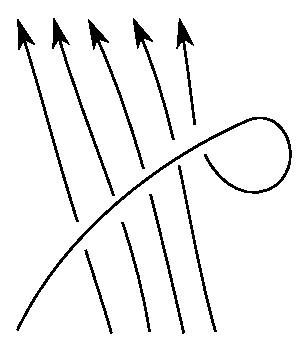
\includegraphics[width=0.2\linewidth]{torusbraid.eps}
    \caption{The diagram $\beta_5$}%
    \label{fig:torusbraid}
\end{figure}
Next, we will consider the diagram $\sigma_m$ below and denote its $n$-th power by $S_m^n$. These are required for the satellite construction for links, but we will not need it here.
\begin{figure}[H]
    \centering
    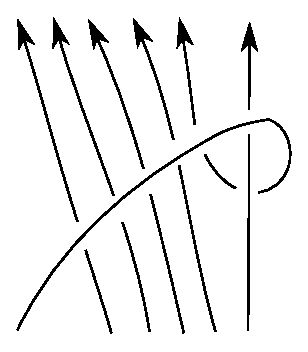
\includegraphics[width=0.2\linewidth]{splicebraid.eps}
    \caption{The diagram $\sigma_5$}%
    \label{fig:splicebraid}
\end{figure}

To conclude this section, we will explain how to actually construct the link diagram in the annulus for a non-reducible singularity. Let $C_1, \ldots, C_r$ be the branches of $C$ at $0$ and consider truncated Puiseux series
\[ y_i(x) = x^{\frac{q^i}{p^i}} (a_i + z_i(x^{\frac{1}{p^i}})). \]
Write $\alpha_i = \frac{q^i}{p^i}$ and consider the pairs $(\alpha_i, a_i)$. It is always possible to find a finite truncation of the Puiseux series that does not affect the topological type of the link, so the inductive process we will define is actually finite. For each $(\alpha, a)$, let $\qty{i_0, \ldots, i_n}$ be the set of indices with associated pair $(\alpha, a)$. Assume we have an annulus diagram $L_{(\alpha, a)}$ and set
\[ L_{\alpha} \coloneqq \prod_a L_{(\alpha, a)}. \]
We may assume that $\alpha_1 < \cdots < \alpha_k$, and the link $\mc{L}_C$ can be represented by the annulus diagram
\[ L_C \coloneqq S_{p^1}^{q^1} * (L_{\alpha_1}, S_{p^2}^{q^2} * (L_{\alpha_2}, \ldots, S_{p^{k-1}}{q^{k-1}} * T_{p^k}^{q^k} * L_{\alpha_k})). \]

\section{Some explicit calculations for the unknot and Hopf link}%
\label{sec:some_explicit_calculations_for_the_unknot_and_hopf_link}

The following is already apparently known.
\begin{prop}
    For any partition $\lambda$, 
    \[ \ev{Q_{\lambda}} = \prod_{\square \in \lambda} \frac{v^{-1} s^{c(\square)} - v s^{-c(\square)}}{s^{h(\square)} - s^{-h(\square)}}. \]
\end{prop}

Let $X \in \mc{C}_+$ be a counterclockwise-oriented diagram. Define the \textit{meridian operator} $\ms{M}_X$ on $\mc{C}_+$ by the construction below:
\begin{figure}[H]
    \centering
    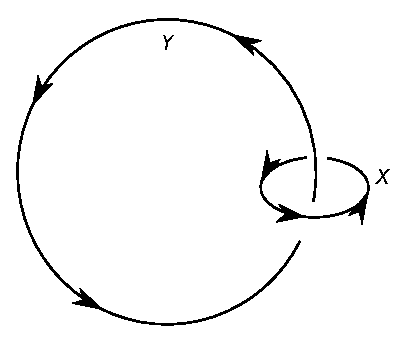
\includegraphics[width=0.2\linewidth]{mer6.eps}
    \caption{Meridian operator}%
    \label{fig:mer6}
\end{figure}
For a partition $\mu$, the Schur function $Q_{\mu}$ is an eigenvector for $\ms{M}_X$ with eigenvalue $t_{\mu}(X)$. Then the HOMFLY polynomial for the colored Hopf link decorated by $\mu, \lambda$ is simply $t_{\mu}(Q_{\lambda})(t_{\mu})$. In the remainder of this section, we will describe the operator $t_{\mu}$, which is a ring homomorphism $\mc{C}_+ \to \Lambda$. Define the function
\[ E_{\mu}(t) = \prod_{j=1}^{\ell(\mu)} \frac{1+v^{-1}s^{\mu_j - 2j + 1}t}{1+v^{-1}s^{-2j+1}t} \prod_{i \geq 0} \frac{1+v s^{2i+1}t}{1+v^{-1}s^{2i+1}t}. \]
Then we have $t_{\mu}(Q_{\lambda}) = s_{\lambda}(E_{\mu}(t))$, where for a power series $E(t) = \sum E_k t^k$, we write $s_{\lambda}$ as a polynomial in the $e_k$ and then substitute $e_k \gets E_k$.

\section{Behavior of links with respect to blowup}%
\label{sec:behavior_of_links_with_respect_to_blowup}

Having discussed the behavior of enumerative invariants with respect to blowups, we need to discuss the behavior of the link $\mc{L}_{C,0}$ with respect to blowing up the origin. Let $C_1, \ldots, C_r$ be the irreducible components of $C$ through $0$ and denote their strict transforms by $C_i'$. At each point $p_1, \ldots, p_e \in E$ (the exceptional divisor) let $D_k$ denote the singularity of $C' \cup E$ at $p_k$ and $B_k$ be the singularity of $C'$ at $p_k$. Choose (truncated) Puiseux expansions
\[ y_i(x) = x^{\frac{q^i}{p^i}} (a_i + z_i (x^{\frac{1}{p^i}})) \]
For each of the branches $C_i$. We may also assume that $\frac{q^i}{p^i} \geq 1$ for all $i$. If we blow up at the origin, consider the chart with coordinates $(x, y = xw)$. Substitution, we obtain the new Puiseux expansion
\[ w_i(x) = x^{\frac{q^i - p^i}{p^i}} (a_i + z_i(x^{\frac{1}{p^i}})) \]
for $C_i'$ at $p_k$. In particular, we obtain the relation
\[ [L_C] = \tau [L_{C'}] \qquad \tau(-) \coloneqq T_1^1 * (-). \]
If we perform deeper analysis, we obtain the following result:

\begin{prop}
    If any $\alpha_i = \frac{q_i}{p_i} > 1$, then we have
    \[ [L_C] = S_1^1 * (L_{B_1} \cdots L_{b_{e-1}}, \tau L_{B_e}). \]
    Otherwise, we have
    \[ [L_C] = S_1^1 * (L_{b_1} \cdots L_{B_e}, \emptyset) = T_1^1 * (L_{B_1} \cdots L_{B_e}). \]
\end{prop}

Now we will write down a blowup identity for links. The idea is to use the topological vertex (originally introduced by Aganagic-Klemm-Marino-Vafa) and its relationship with Chern-Sinons invariants of the unknot. For a partition $\mu$, define
\begin{align*}
    Z_{\mu}(q, Q) &= s_{\mu}(q^{\rho}) \prod_{\square \in \mu} (1 + Q q^{-c(\square)}) \\
    &= q^{\kappa_{\mu}/4} \prod_{\square \in \mu} \frac{1 + Q q^{-c(\square)}}{q^{h(\square)/2} - q^{-h(\square)/2}}.
\end{align*}
Here, $\kappa_{\mu} = 2 \sum_{\square \in \mu} c(\square)$. By the computation of the colored HOMFLY polynomial of the colored unknot (sorry), we obtain the identity
\begin{align*}
    Z_{\mu}(q=s^2, Q=-v^2) = v^{\abs{\mu}} \ev{Q_{\mu}}.
\end{align*}

\section{Relation between PT theory and HOMFLY}%
\label{sec:relation_between_pt_theory_and_homfly}

We will prove a relationship between the PT partition function for $C$-framed stable pairs in $Y = \mc{O}_{\P^1}(1) \oplus \mc{O}_{\P^1}(1)$ and the HOMFLY polynomial for $\mc{L}_{C,0}$. We will focus on the simplest case of a node with two branches. The general case reduces to this one by careful checking of what happens on both sides under blowup of $C$ at $0$.

\begin{prop}
    We have the identity (possibly up to monomials)
    \[ \ms{Z}'(Y, C; q, Q=0) = {(-1)}^{\ep} s^b \ev{[L_C * Q_{{(1)}^t}]}^{\mr{low}}, \]
    where the superscript low means we take the lowest degree terms.
\end{prop}

We only need to prove this for the unknot and the Hopf link.

\begin{proof}
    This apparently follows from the fact that the topological vertex calculates both the $v=0$ specialization of HOMFLY of the Hopf link and the stable pairs vertex. See the references to Maulik's paper for a reference.
\end{proof}





\end{document}
